% http://tex.stackexchange.com/questions/11866/compile-a-latex-document-into-a-png-image-thats-as-short-as-possible#11880
%http://tex.stackexchange.com/questions/152247/best-practice-to-include-standalone-precompiled-graphics
\documentclass[border=1pt]{standalone}
\usepackage{tikz}

\begin{document}

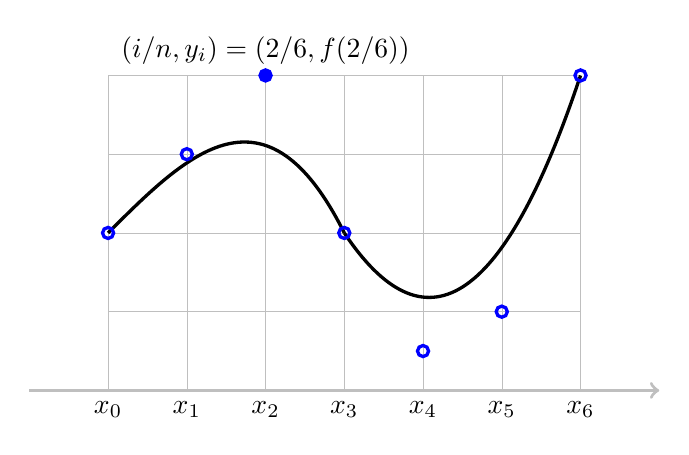
\begin{tikzpicture}[very thick]
	\coordinate (A1) at (0,0);
	\coordinate (A2) at (6, 4);
	\draw [help lines, lightgray] (A1) grid (A2);
	\draw [->, lightgray] (-1, 0) -- (7, 0);

	\newcommand*{\n}{-2.5}
	
		\draw (0,2) .. controls (1,3) and (2,4) .. (3,2);
		\draw (3,2) .. controls (4,0.5) and (5,1) .. (6,4);

	\foreach \x / \y in {0/2,1/3,2/4,3/2,4/0.5,5/1,6/4}{
		\draw[blue] (\x,\y) circle (2pt);
	\node[below] (\x) at (\x,0) {$x_\x$};}


		\fill[blue] (2,4) circle (2pt);
		\node[above] at (2,4) {$(i/n,y_i) = (2/6, f(2/6))$};

\end{tikzpicture}

\end{document}
